\chapter{Results}


\section{Results of various oversamplings and undersamplings}
This simple two-dimensional data can be visualized. 

\subsection{Visualizing Simple 2D Data Set}
\subsubsection{Visualizing The Data Set}
Visualize a simple two-dimensional dataset that has been created.

\begin{center}
    \begin{figure*}[ht]
        \caption{Visualizing Simple 2D Data Set: Do Nothing Before Training}
        \label{tab:team-rating-features}
        \begin{center}
            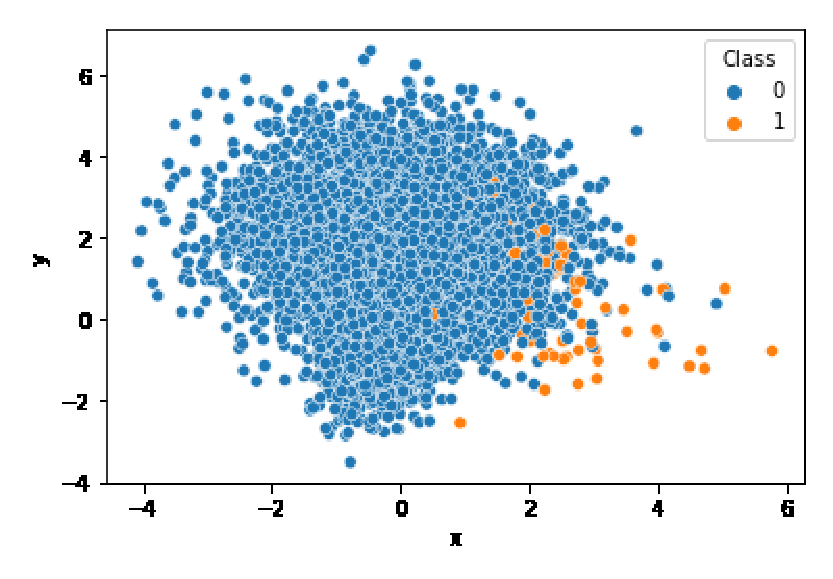
\includegraphics[scale=0.6]{image/no-prepro.eps}
        \end{center}
    \end{figure*}
\end{center}

\clearpage
\subsubsection{Visualizing SMOTE}
As a preprocessing step, using SMOTE , and the data set looked like this.

\begin{center}
    \begin{figure*}[ht]
        \caption{Visualizing Simple 2D Data Set: SMOTE}
        \label{tab:team-rating-features}
        \begin{center}
            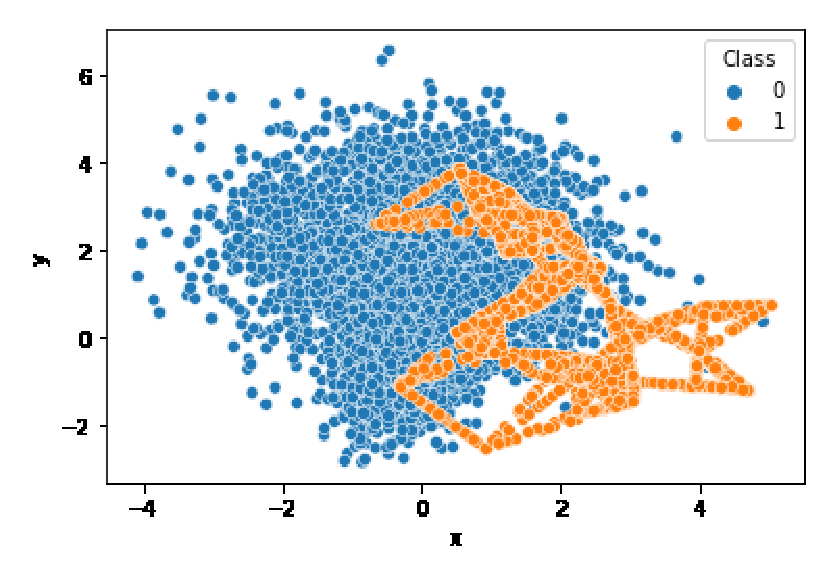
\includegraphics[scale=0.6]{image/smote.eps}
        \end{center}
    \end{figure*}
\end{center}

The linearly increasing data set shows the characteristics of the minority data.

\clearpage
\subsubsection{Visualizing Tomek Links}
Using undersampling with Tomek Links as preprocessing, the data set looked like this

\begin{center}
    \begin{figure*}[ht]
        \caption{Visualizing Simple 2D Data Set: Tomek Links}
        \label{tab:team-rating-features}
        \begin{center}
            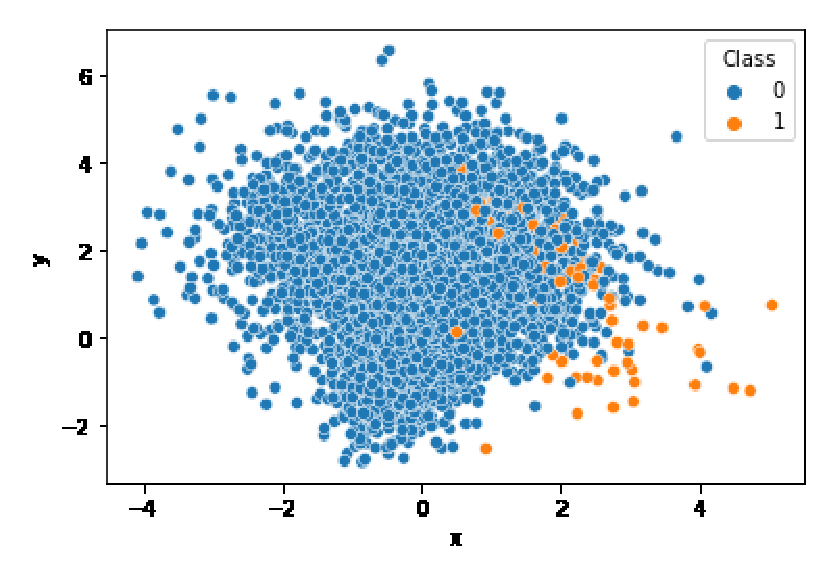
\includegraphics[scale=0.6]{image/tomek-links.eps}
        \end{center}
    \end{figure*}
\end{center}

I was not able to capture the features very effectively. It may have been due to too much bias.

\clearpage
\subsubsection{Visualizing Smote and Tomek Links Combine}
With both Smote and undersampling using Tomek Links as preprocessing, the data set looked like this
\begin{center}
    \begin{figure*}[ht]
        \caption{Visualizing Simple 2D Data Set: Smote and Tomek Links Combine}
        \label{tab:team-rating-features}
        \begin{center}
            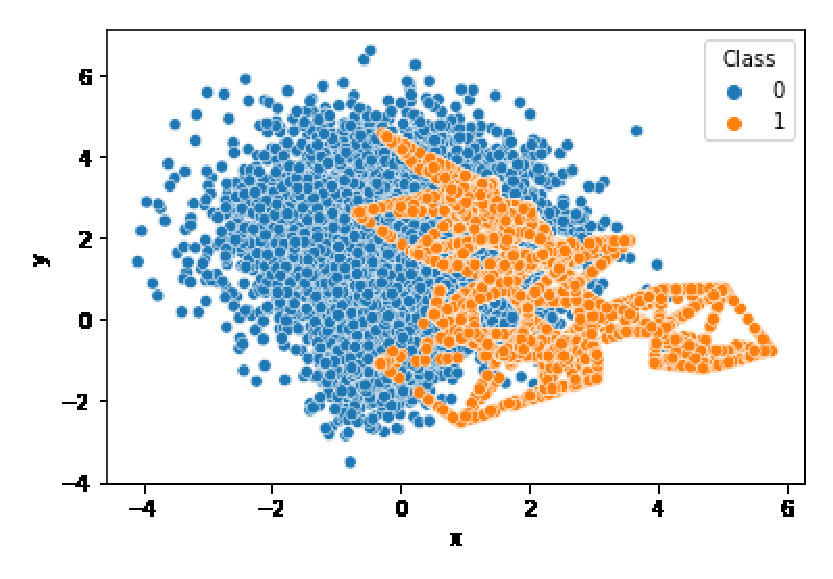
\includegraphics[scale=0.6]{image/combine.eps}
        \end{center}
    \end{figure*}
\end{center}

A few are strongly characterized by data that are not only linear. It is thought that they appear more effectively when combined.

\clearpage
\subsubsection{Visualizing MySMOTE}
When using MySMOTE instead of Smote as preprocessing, the data set looked like this.

\begin{center}
    \begin{figure*}[ht]
        \caption{Visualizing Simple 2D Data Set: MySMOTE}
        \label{tab:team-rating-features}
        \begin{center}
            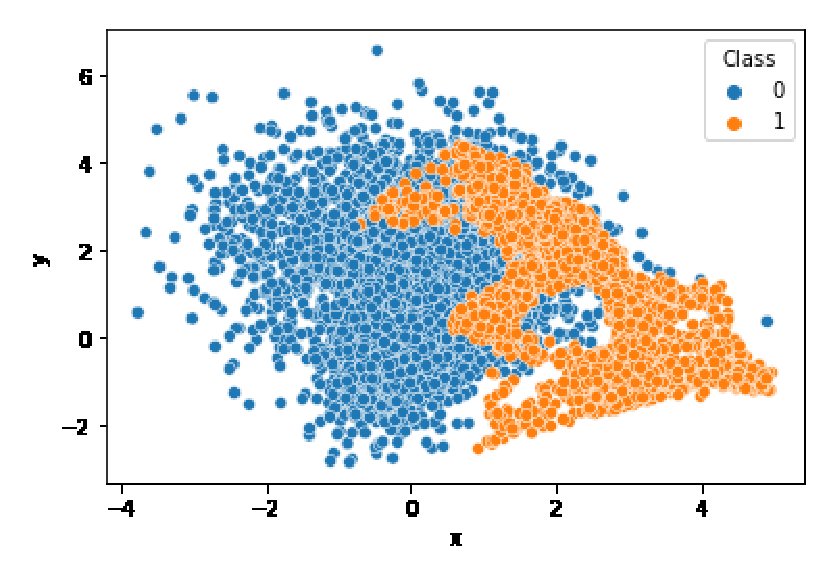
\includegraphics[scale=0.6]{image/mysmote.eps}
        \end{center}
    \end{figure*}
\end{center}

\clearpage

\subsection{Classification results}
\subsubsection{Simple 2D Data Set}
The actual results of adapting the model are shown below.
\begin{table}[H]
    \caption{Classification Result Simple 2D Dataset Table}
    \centering
    \begin{tabular}{|l|l|l|l|l|}
    \hline
         & Accuracy & precision & recall & AUC \\ \hline
        Without Pretreatment & 0.99100 & 0.6250 & 0.1724 & 0.58570 \\ \hline
        Using SMOTE & 0.92800 & 0.1055 & 0.8621 & 0.89536 \\ \hline
        Using Tomek-links & 0.99133 & 0.7143 & 0.1724 & 0.58587 \\ \hline
        Using Combine & 0.91500 & 0.0935 & 0.8966 & 0.90587 \\ \hline
        Using MySMOTE & 0.93233 & 0.1116 & 0.8621 & 0.89754 \\ \hline
    \end{tabular}
\end{table}


\subsubsection{German Credit Dataset}

\begin{table}[H]
    \caption{Classification Result German Credit Dataset}
    \centering
    \begin{tabular}{|l|l|l|l|l|}
    \hline
         & Accuracy & precision & recall & AUC \\ \hline
        Without Pretreatment & 0.68667 & 0.4500 & 0.5357 & 0.64054 \\ \hline
        Using SMOTE & 0.72333 & 0.5364 & 0.6484 & 0.70217 \\ \hline
        Using Tomek-links & 0.75000 & 0.6600 & 0.3626 & 0.64065 \\ \hline
        Using Combine & 0.68333 & 0.4861 & 0.7692 & 0.70758 \\ \hline
        Using MySMOTE & 0.63000 & 0.4026 & 0.7654 & 0.67267 \\ \hline
    \end{tabular}
\end{table}


\subsubsection{Haberman's Survival Data Set}

\begin{table}[H]
    \caption{Classification Result Haberman's Survival Dataset}
    \centering
    \begin{tabular}{|l|l|l|l|l|}
    \hline
         & Accuracy & precision & recall & AUC \\ \hline
        Without Pretreatment & 0.76087 & 0.6000 & 0.2500 & 0.59559 \\ \hline
        Using SMOTE & 0.59783 & 0.3488 & 0.6250 & 0.60662 \\ \hline
        Using Tomek-links & 0.76087 & 0.5556 & 0.4167 & 0.64951 \\ \hline
        Using Combine & 0.71739 & 0.4737 & 0.7500 & 0.72794 \\ \hline
        MySMOTE & 0.68478 & 0.4118 & 0.6087 & 0.65942 \\ \hline
    \end{tabular}
\end{table}

\subsubsection{Census-Income (KDD) Data Set}

\begin{table}[H]
    \caption{Classification Result Census-Income (KDD) Data Set}
    \centering
    \begin{tabular}{|l|l|l|l|l|}
    \hline
         & Accuracy & precision & recall & AUC \\ \hline
        Without Pretreatment & 0.84553 & 0.8618 & 0.9503 & 0.72808 \\ \hline
        Using SMOTE & 0.83816 & 0.8743 & 0.9206 & 0.74578 \\ \hline
        Using Tomek-links & 0.84553 & 0.8618 & 0.9503 & 0.72808 \\ \hline
        Using Combine & 0.73928 & 0.8948 & 0.7466 & 0.73109 \\ \hline
        MySMOTE & 0.84584 & 0.8624 & 0.9491 & 0.73248 \\ \hline
    \end{tabular}
\end{table}


\subsubsection{Blood Transfusion Service Center Data Set}

\begin{table}[H]
    \caption{Classification Result Blood Transfusion Service Center Data Set}
    \centering
    \begin{tabular}{|l|l|l|l|l|}
    \hline
         & Accuracy & precision & recall & AUC \\ \hline
        Without Pretreatment & 0.77778 & 0.6333 & 0.3276 & 0.63086 \\ \hline
        Using SMOTE & 0.74222 & 0.5000 & 0.4483 & 0.64629 \\ \hline
        Using Tomek-links & 0.77778 & 0.6333 & 0.3276 & 0.63086 \\ \hline
        Using Combine & 0.65333 & 0.4324 & 0.7619 & 0.68651 \\ \hline
        MySMOTE & 0.69333 & 0.4667 & 0.6667 & 0.68519 \\ \hline
    \end{tabular}
\end{table}
